\documentclass[UTF8]{ctexart}
\ctexset { section = { format={\Large \bfseries } } }
\pagestyle{plain}
\usepackage{float}
\usepackage{amsmath}
\usepackage{amssymb}
\usepackage{listings}
\usepackage{graphicx}%插入图片宏包
\usepackage{xcolor}
\usepackage{geometry}
\geometry{a4paper,scale=0.8}
\usepackage{caption}
\usepackage{subcaption}
\usepackage[colorlinks=true, linkcolor=blue, citecolor=blue, urlcolor=blue]{hyperref}
\captionsetup[figure]{name={Figure}}
\captionsetup[table]{name={Table}}
\definecolor{Rhodamine}{RGB}{227,11,92}


\lstset{
language=Python, % 设置语言
basicstyle=\ttfamily\small, % 设置字体族
breaklines=true, % 自动换行
keywordstyle=\bfseries\color{blue}, % 设置关键字为粗体,
morekeywords={}, % 设置更多的关键字,用逗号分隔
emph={self}, % 指定强调词,如果有多个,用逗号隔开
emphstyle=\bfseries\color{Rhodamine}, % 强调词样式设置
commentstyle=\color{black!50!white}, % 设置注释样式,斜体,浅灰色
stringstyle=\bfseries\color{red!90!black}, % 设置字符串样式
columns=flexible,
numbers=left, % 显示行号在左边
numbersep=2em, % 设置行号的具体位置
numberstyle=\footnotesize, % 缩小行号
frame=single, % 边框
framesep=1em % 设置代码与边框的距离
}

\title{\textbf{Image Processing Homework 6}}
\author{吴嘉骜 21307130203}
\date{\today}

\begin{document}

\maketitle

\noindent
\section{}
\setlength{\parindent}{0pt}
Implement a segmentation algorithm using either K-means clustering or a Gaussian Mixture Model (choose one, and do not use functions from external libraries).\\
Test the algorithm on images contaminated with noise (e.g., 0.1\% salt-and-pepper noise):

(1)Test binary segmentation and compare the results of your implemented algorithm with those obtained using a thresholding method (such as Otsu's method or based on maximum entropy).

(2)Test multi-class segmentation (please decide the number of segmentation label classes yourself, with at least three classes).

(3)Discuss why the segmentation results are inaccurate for noisy images and what methods might yield better segmentation results (note: you are not required to implement these methods, just discuss them).

\textbf{Solution}:\\
For $\textit{GMMEM}$, the code in \texttt{gmmem.py} depends largely on the slides despite some modifications, and thus shown in the \hyperlink{code1}{Appendix}.
The code for $\textit{K-means}$ is in \texttt{kmeansimg.py} is shown below.\\
\begin{lstlisting}
from PIL import Image
import numpy as np
import matplotlib.pyplot as plt
def kmeans(img, k, max_iter=100, tol=1e-5):
    '''
    Use k-means algorithm to segment the image.
    '''
    # Initialize the centroids by selecting k random pixels from the image
    np.random.seed(7)  # for reproducibility
    centroids = img.ravel()[np.random.choice(img.size, k, replace=False)]

    height, width = img.shape
    labels = np.zeros((height, width), dtype=np.int_)

    m = 0  # Number of iterations
    for _ in range(max_iter):
        # Update the labels
        distances = (img[..., None] - centroids)**2  # broadcasting to subtract centroids from all pixels
        labels = np.argmin(distances, axis=2)  # find the index of the closest centroid

        # Update the centroids
        centroids_new = np.array(
            [img[labels == i].mean() if np.any(labels == i) else 0 for i in range(k)])  # avoid empty clusters

        # Check the convergence
        if np.sqrt(np.sum((centroids_new - centroids)**2)) < tol:
            print('Kmeans Converged! Number of iteration: ', m)
            break
        else:
            centroids = centroids_new
            m += 1

    new_img = np.zeros((height, width), dtype=np.uint8)
    for i in range(k):
        new_img[labels == i] = centroids[i]

    return labels, centroids, new_img
\end{lstlisting}
For $\textit{K-means}$, we first initialize the centroids by randomly selecting $k$ pixels from the image.
Then we update the labels by assigning each pixel to the closest centroid. We then update the centroids by calculating the mean of the pixels in each cluster.
The procedure is repeated until the centroids converge or the maximum number of iterations is reached.\\
For $\textit{GMMEM}$, we first initialize the parameters $\pi_k$ with equal weights, $\mu_k$ as the centroids obtained from $\textit{K-means}$,
and $\sigma_k^2$ as the global variance of the image. Then we perform E-step and M-step alternatively until the parameters converge or the maximum number of iterations is reached.\\

\textbf{Result}:\\
We test the $\textit{K-means}$ and $\textit{GMMEM}$ segmentation on an image polluted with salt-and-pepper noise, and the result is shown in Figure \ref{fig:seg}.\\
\begin{figure}[htbp]
    \centering
    \begin{subfigure}{0.3\textwidth}
        \centering
        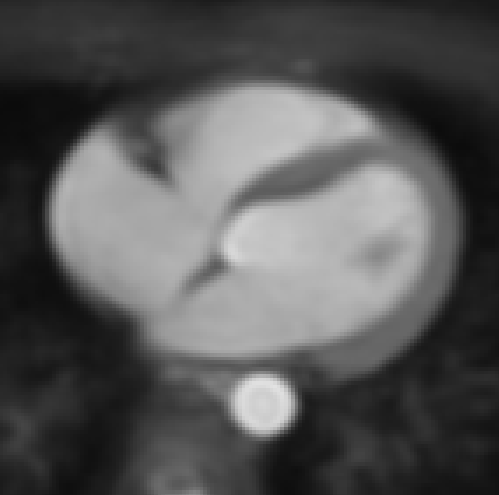
\includegraphics[width=0.8\linewidth]{heartimg.png}
        \caption{Original image}
    \end{subfigure}%
    \hfill
    \begin{subfigure}{0.3\textwidth}
        \centering
        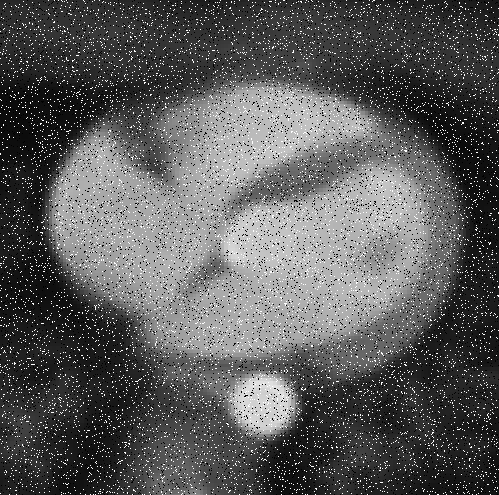
\includegraphics[width=0.8\linewidth]{heart_noised.png}
        \caption{Salt-and-pepper noise, $p=0.1$}
    \end{subfigure}%
    \hfill
    \begin{subfigure}{0.3\textwidth}
        \centering
        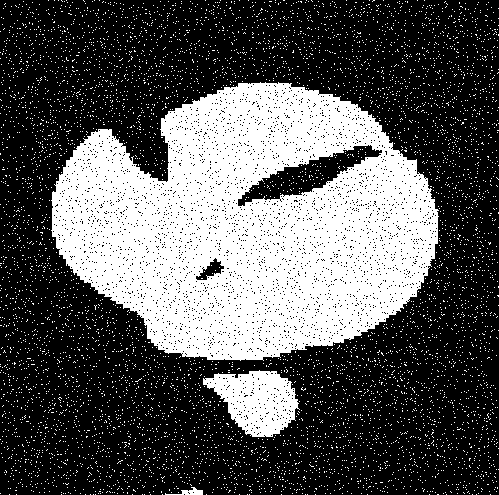
\includegraphics[width=0.8\linewidth]{heart_otsu.png}
        \caption{Otsu's thresholding}
    \end{subfigure}

    \vspace{0.5cm}
    \centering
    \begin{subfigure}{0.2\textwidth}
        \centering
        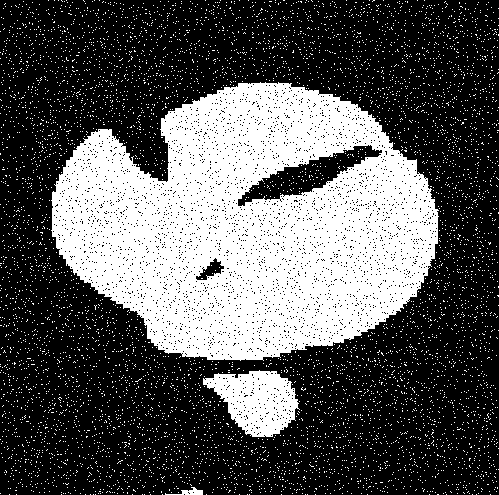
\includegraphics[width=\linewidth]{heart_kmeans2.png}
        \caption{K-means segmentation, $K=2$}
    \end{subfigure}%
    \hfill
    \begin{subfigure}{0.2\textwidth}
        \centering
        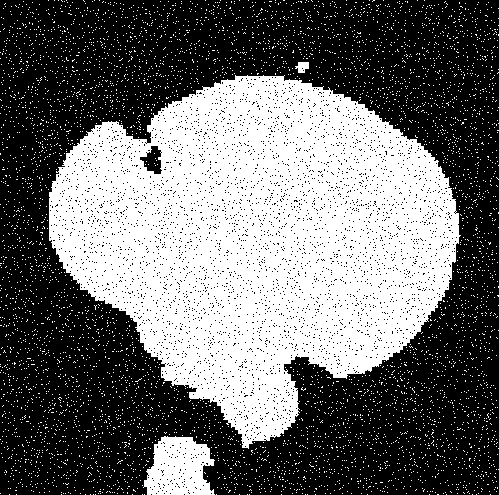
\includegraphics[width=\linewidth]{heart_gmm2.png}
        \caption{GMMEM segmentation, $K=2$}
    \end{subfigure}%
    \hfill
    \begin{subfigure}{0.2\textwidth}
        \centering
        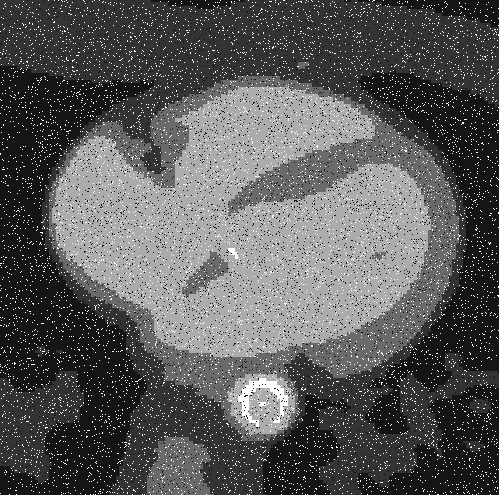
\includegraphics[width=\linewidth]{heart_kmeans5.png}
        \caption{K-means segmentation, $K=5$}
    \end{subfigure}%
    \hfill
    \begin{subfigure}{0.2\textwidth}
        \centering
        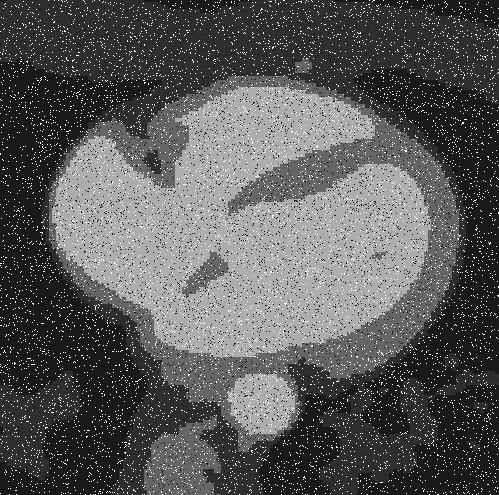
\includegraphics[width=\linewidth]{heart_gmm5.png}
        \caption{GMMEM segmentation, $K=5$}
    \end{subfigure}
    \caption{Heart image segmentation}
    \label{fig:seg}
\end{figure}

\textbf{Analysis}:\\
(1) For binary segmentation, I find that the segmentation result of $\textit{K-means}$ is similar to that of Otsu's method, whereas the performance of $\textit{GMMEM}$ is not as optimal as the other two,
because it tends to segment the main part of the heart as a single class, which deviates from our desired outcome. Also, running $\textit{GMMEM}$
is rather slow and seems not to converge within maximum iterations.
The conditions for covergence may be a little strict. 

(2) In multi-class segmentation, the performance of $\textit{GMMEM}$ surpasses that of $\textit{K-means}$. 
The processed image is much closer to the original, but there is still room for improvement due to the presence of unremoved noise.

(3) The inaccuracy in segmentation results for noisy images stems from our algorithm's inability to effectively recognize and handle noise. 
I used salt-and-pepper noise, which is sharp and sudden disturbances in the image. 
This type of noise can significantly alter the pixel intensity distribution, making traditional segmentation algorithms less effective, as they often rely on these distributions.\\
Before segmentation, using smoothing methods that are less sensitive to outliers such as the median filter can help in reducing the effect of salt-and-pepper noise.
Adaptive thresholding may also be applied to improve the segmentation results, as it can automatically adjust the threshold  over different parts of the image.
Additionallly, pre-processing techniques like morphological operations (erosion and dilation) can help in reducing the noise. 

\section{}
Use morphological operations learned in the course to implement hole filling and removal of isolated points in binary images.\\
You should code the morphological operations yourself and not use library functions.\\

\textbf{Solution}:\\
The morphological methods are implemented in \texttt{morph.py}, and is shown below.\\
\begin{lstlisting}
from PIL import Image
import numpy as np
import matplotlib.pyplot as plt

def dilation(image, kernel):
    k_h, k_w = kernel.shape
    i_h, i_w = image.shape

    # calculate padding size
    pad_height = k_h // 2
    pad_width = k_w // 2

    # padding image
    padded_image = np.pad(image, ((pad_height, pad_height), (pad_width, pad_width)), mode='constant')
    dilated_image = np.zeros_like(image)
    for i in range(i_h):
        for j in range(i_w):
            # the neighborhood of the current pixel
            neighborhood = padded_image[i:i+k_h, j:j+k_w]
            # apply dilation operation
            dilated_image[i, j] = np.max(neighborhood * kernel)

    return dilated_image

def erosion(image, kernel):
    k_h, k_w = kernel.shape
    i_h, i_w = image.shape

    # calculate padding size
    pad_height = k_h // 2
    pad_width = k_w // 2

    # padding image
    padded_image = np.pad(image, ((pad_height, pad_height), (pad_width, pad_width)), mode='constant')
    eroded_image = np.zeros_like(image)
    for i in range(i_h):
        for j in range(i_w):
            # the neighborhood of the current pixel
            neighborhood = padded_image[i:i+k_h, j:j+k_w]
            # apply erosion operation
            eroded_image[i, j] = np.min(neighborhood[kernel == 1])

    return eroded_image

def opening(image, kernel1, kernel2):
    return dilation(erosion(image, kernel1), kernel2)

def closing(image, kernel1, kernel2):
    return erosion(dilation(image, kernel1), kernel2)
\end{lstlisting}
\newpage
For dilation, we construct a kernel with odd size and apply it to every pixel in the image.
The kernel is a matrix with 0 and 1, and the size of the kernel is the size of the neighborhood.
To avoid the boundary problem, we pad the image with 0 ahead of time.
The kernel is applied to the neighborhood of the current pixel, and the intensity is set to white 
if there is at least one white pixel in the neighborhood overlapping with the "1"s in the kernel.
This is equivalent to obtain the maximum intensity where the kernel overlaps with the neighborhood in binary images.\\
For erosion, the procedure is similar, with the only differnce that the intensity is set to white only when
all the pixels in the neighborhood overlapping with "1"s in the kernel are white. 
This is equivalent to obtain the minimum intensity as described above.\\
Opening is the erosion followed by dilation, and closing is the dilation followed by erosion.\\

\textbf{Result}:\\
We test the morphological operations on the given binary image and the result is shown in Figure \ref{fig:morph}.\\
\begin{figure}[htbp]
    \centering
    \begin{subfigure}{0.5\textwidth}
        \centering
        
\includegraphics[width=\linewidth]{zmic_fdu.png}
        \caption{Original image}
    \end{subfigure}%
    \hfill
    \begin{subfigure}{0.5\textwidth}
        \centering
        
\includegraphics[width=\linewidth]{zmic_fdu_noise.png}
        \caption{Image with noise}
    \end{subfigure}%

    \vspace{0.5cm}
    \centering
    \begin{subfigure}{0.5\textwidth}
        \centering
        
\includegraphics[width=\linewidth]{zmic_fdu_clear.png}
        \caption{Opening with kernel $5\times 5$ and  $9\times 9$}
    \end{subfigure}%
    \hfill
    \begin{subfigure}{0.5\textwidth}
        \centering
        
\includegraphics[width=\linewidth]{zmic_fdu_clear1.png}
        \caption{Closing with kernel $5\times 5$ and  $9\times 9$}
    \end{subfigure}%
    \caption{Morphological operations}
    \label{fig:morph}
\end{figure}

\textbf{Analysis}:\\
The morphological operations are effective in removing noise and filling holes in the image.
After some trials, I found that dilation operation could remove the noise points and lines,
while erosion operation could fill the holes in the image. This is aligned with theoretical analysis since
our image is black in the foreground and white in the background.
In addition, the kernel sizes for both operations have to be larger than $5 \times 5$ to achieve desired results.\\
Then we can combine the two operations to obtain better results. The second line above shows the result of opening and closing.
I find that both operations with kernel $5\times 5$ and thereafter $9\times 9$ can reach a desired outcome.
We can notice that the left result (opening) proves better, as there are still some gaps in the letter "D" in the right result.
The reason is probably that the noises are far from the letters, but some holes are closer to the background.
If we first remove the noises by dilation, some letter boundary may be removed as well, and it is difficult to recover by erosion,
as shown in the right result. Also due to padding, there is a black frame around the image. However, first filling the holes by erosion
will not much affect the letters, and then dilation to remove the noises will give a nice result.

\newpage
\appendix
\hypertarget{code1}{\section{Code for GMMEM}}
\begin{lstlisting}
from PIL import Image
import numpy as np
import matplotlib.pyplot as plt
from kmeansimg import kmeans

class Gmmem():
    def __init__(self, img, k, paras):
        self.img = img  # Image to be segmented
        self.num = k  # Number of classes
        self.shape = img.shape  # Shape of the image
        # Parameters for the GMM, including the weights(\pi_k), means(\mu) and variances(\sigma^2)
        self.paras = paras

    def phi(self, mean, var, x):
        # Normal probability density function
        return np.exp(-(x - mean) ** 2 / (2 * var)) / np.sqrt(2 * np.pi * var)

    def get_prob(self, x):
        # Calculate the posterior probability for each class and return the class with the highest probability
        prob = np.array([self.phi(self.paras[1][i], self.paras[2][i], x) for i in range(self.num)])
        posterior = (prob * self.paras[0]) / \
            (np.sum(prob * self.paras[0]) + 1e-8)  # avoid zero division
        return int(np.argmax(posterior))

    def inference(self):
        # Perform inference on the image, and return the mask with the same shape as the image
        mask = np.array([self.get_prob(i) for i in self.img.reshape(-1)]
                        ).reshape(self.shape[0], self.shape[1])
        return mask

    def segmentation(self, max_iter=30, tol=1e-3):
        # Perform segmentation on the image, alternatively perform E-step and M-step
        m = 0  # Number of iterations
        while True:
            P = self.E_step()  # E-step: Calculate posterior probabilities
            # M-step: Update model parameters
            new_paras = self.M_update_paras(P)
            # if ((new_paras - self.paras) < tol).all:
            #     print('gmm Converged! Number of iteration: ', m)
            #     break
            if np.sqrt(np.sum((new_paras - self.paras)**2)) < tol:
                print('gmm Converged! Number of iteration: ', m)
                break
            elif m > max_iter:
                break
            else:
                self.paras = new_paras
                m += 1
        mask = self.inference()
        return mask

    def P_cal(self, x):
        # Calculate Q/posterior for every pixel
        prob = np.array([self.phi(self.paras[1][i], self.paras[2][i], x)
                        for i in range(self.num)])
        posterior = (prob * self.paras[0]) / \
            (np.sum(prob * self.paras[0]) + 1e-8)  # avoid zero division
        return posterior

    def E_step(self):
        # Calculate the posterior probabilities for each pixel in the image
        P = np.stack([self.P_cal(i)
                    for i in self.img.reshape(-1)], 0).T  # (k, h*w)
        return P

    def M_update_paras(self, P):
        # Update the model parameters based on the posterior probabilities
        new_paras = np.zeros(self.paras.shape)
        new_paras[1] = np.array(
            [np.sum(P[i] * self.img.reshape(-1)) / np.sum(P[i]) for i in range(self.num)])
        new_paras[2] = np.array([np.sum(P[i] * (self.img.reshape(-1) - new_paras[1][i]) ** 2) / np.sum(P[i]) for i in range(self.num)])
        new_paras[0] = np.sum(P, -1) / np.sum(P)
        new_paras[2][new_paras[2] < 1] = np.random.randint(1, 10, 1)  # Avoid zero variance
        return new_paras
    
    def create_newimg(self, max_iter=30, tol=1e-3):
        # Create a new image based on the labels
        labels = self.segmentation(max_iter, tol)
        new_img = np.zeros(self.shape, dtype=np.uint8)
        for i in range(self.num):
            new_img[labels == i] = self.paras[1][i]
        return new_img
    
def initialize_paras(img, k):
    paras = np.zeros((3, k))
    paras[0] = np.ones(k) / k  # equal weights
    labels, centroids, _ = kmeans(img, k)
    paras[1] = centroids
    paras[2] = np.array([np.var(img[labels == i]) for i in range(k)])
    return paras
\end{lstlisting}
\end{document}